\begin{mainquestion}{zenerregulator}{Zener Diode Voltage Regulator Design}

As a consultant, you are hired to evaluate a zener diode in a power supply that attempts to provide $v_L$ between 5.1 V and 5.5 V for a USB accessory. Your client's proposed circuit is shown to the right. The source voltage $V_s$ is known to vary between 6.8 and 11.2 V. Experiments show the load current $i_L$ can vary from 0 to 100 mA.

\begin{center}
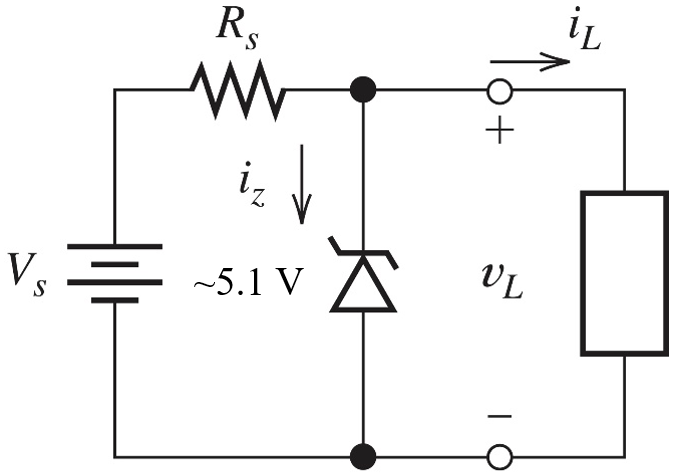
\includegraphics[width=3.5in]{zener_circuit.png}
\end{center}

% =========================================================
\begin{partquestion}{inadequatedesign}
{Initially you are told that $R_s = \qty{100}{\ohm}$. Show it is not possible to maintain $v_L$ in the desired range considering the range of fluctuating circuit parameters provided.}

\begin{answer}
The zener diode can maintain the desired voltage as long as we keep it in breakdown mode. This is possible unless the voltage drop across the resistor is such that the zener diode voltage drops under its rated breakdown value. In equation form:

\[
v_L = V_s - (i_z + i_L) R_s
\]

This is lowest when $V_s$ is at its minimum value, and when $i_L$ is at its maximum value. Plugging in these given values leads to:

\begin{align*}
v_L &= 6.8 - (i_z + 0.1) 100 \\
&= -3.2 - 100i_z
\end{align*}

which will be much less than the desired voltage level near 5.1 V. (Note that $i_z$ is non-negative; it is zero when the diode is not conducting and some positive value when it is operating in breakdown mode.) Clearly this value of resistor is too large!
\end{answer}
\end{partquestion}

% =========================================================
\begin{partquestion}{maxresistor}
{What is the maximum value of $R_s$ that prevents $v_L$ from dropping below the desired range if the zener diode breakdown voltage is $V_{Z0} = \qty{5.1}{\volt}$ (an industry standard value)?}

\begin{answer}
We can reuse the formula from the previous part:

\[
v_L = V_s - (i_z + i_{L,\max}) R_s
\]

and consider the case where we are in breakdown, such that $v_L \geq V_{Z0} = \qty{5.1}{\volt}$. We have:

\begin{align*}
V_{s,\text{min}} - (i_z + i_{L,\max}) R_s &\geq V_{Z0} \\
V_{s,\text{min}} - i_{L,\max} R_s &\geq V_{Z0} \\
R_s &\leq \frac{V_{s,\text{min}} - V_{Z0}}{i_{L,\max}} = \frac{6.8 - 5.1}{0.1} \\
R_s &\leq \qty{17}{\ohm}
\end{align*}

\end{answer}
\end{partquestion}

% =========================================================
\begin{partquestion}{zenercurrent}
{With your updated $R_s$, what is $i_z$ when $V_s$ is at a maximum and the current load is zero?}

\begin{answer}
When the current load is zero, the load is an open circuit and all the current will flow through the zener diode. We can calculate:

\begin{align*}
i_z &= \frac{V_{s,\text{max}} - V_{Z0}}{R} \\
&= \frac{11.2 - 5.1}{17} = \qty{0.359}{\ampere}
\end{align*}

\end{answer}
\end{partquestion}

\end{mainquestion}
